\chapter{Búsqueda de SUSY con producción electrodébil en estados finales con fotones, bosones $Z$ y Higgs}
% \addcontentsline{toc}{chapter}{Búsqueda de SUSY con producción electrodébil}
\chaptermark{Búsqueda de SUSY con producción electrodébil en estados finales con fotones, bosones $Z$ y Higgs}



Es posible realizar una búsqueda alternativa con el mismo estado final, para realizar un búsqueda de un modelo supersimétrico similar al anterior pero dedicado a la preducción electrodébil de partículas de SUSY.

El estado final esta motivado por modelos de supersimetría (SUSY) \cite{Golfand:1971iw, Volkov:1973ix, Wess:1974tw, Wess:1974jb, Ferrara:1974pu, Salam:1974ig, Martin:1997ns}, que son candidatos teóricamente bien motivados para la física más allá del Modelo Estándar (SM). Teorías de ruptura de simetría gauge mediated (GMSB) \cite{Dine:1981gu, AlvarezGaume:1981wy, Nappi:1982hm} predicen un sector oculto en el que la supersimetría se rompe con un valor de expectación de vacío $ \langle F \rangle $, donde la ruptura de simetría se transfiere al sector visible a través de interacciones de bosones gauge del modelo estándar. La partícula supersimétrica más ligera (LSP) en GMSB es el gravitino ultraligero (\gravino), que en determinadas circunstancias es un candidato viable a materia oscura \cite{Goldberg:1983nd, Ellis:1983ew}. La fenomenología de los modelos GMSB está determinada por la naturaleza de la partícula supersimétrica próxima a la más ligera (NLSP), que para una gran parte del espacio de parámetros del GMSB es el neutralino \ninoone. Los neutralinos son mezclas de autoestados de gauginos neutros ($\tilde{B}$, $\tilde{W}^{0}$) y higgsinos neutros ($\tilde{H}^{0}_{u},\tilde{H}^{0}_{d}$), y por lo tanto el neutralino más ligero puede decar a un \gravino by a $\gamma$, $Z$ o $h$ (el bosón de Higgs neutro más ligero, asumido compatible con el bosón de Higgs observado en ATLAS y CMS). Los dos últimos están sujetos a una fuerte supresión cinemática proporcional a $ (1-m_{Z}^{2}/m_{\ninoone}^{2})^4$ y $(1-m_{h^{0}}^{2}/m_{\ninoone}^{2})^4$, pero que aún juegan un papel importante en la fenomenología si $ \langle F \rangle $ no es demasiado grande, \ninoone\ tiene un contenido considerable de zino o higgsino y $m_{\ninoone}$ es significativamente mayor que $m_{Z}$ o $m_{h^{0}} $. Teóricamente se permiten las desintegraciones a \Azero o \Hzero \, pero es poco probable que se permitan cinemáticamente.

En consecuencia, un par de \ninoone\  producidos en un colisionador puede dar lugar a un estado final que contenga dos bosones ($hh$, $h\gamma$, $hZ$, $Z\gamma$, $ZZ$, $\gamma\gamma$) más \met\ de las partículas LSP estables e indetectables (\gravino). Se han realizado varias búsquedas de estas signaturas \cite{SUSY-2011-12, SUSY-2012-12,EXOT-2010-06,SUSY-2011-04,ATLAS-CONF-2012-144,CMS-SUS-10-002 ,CMS-SUS-11-002,CMS-SUS-14-009,SUSY-2014-01,CMS-SUS-14-004,SUSY-2014-08}.
Los escenarios considerados en este análisis son aquellos con al menos un fotón
más dos \gravino\ en el estado final, esperados en el caso en que el \ninoone\ sea una mezcla bino-higgsino, como se muestra en la Figura \ref{fig:GGM_diagrams}.

\begin{figure}
  \centering
  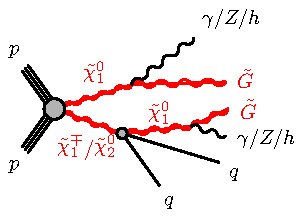
\includegraphics[width=0.3\textwidth]{images/N1N2C1-qqZhphGG-GGM.pdf}%
  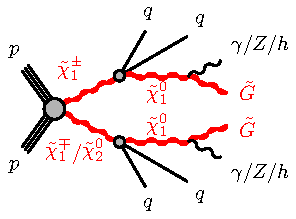
\includegraphics[width=0.3\textwidth]{images/C1C1N2-qqqqZhphGG-GGM.pdf}
  \caption{Diagramas de producción de gauginos con estado final de fotones y gravitinos.}
  \label{fig:GGM_diagrams}
\end{figure}

Los esfuerzos para formular al GMSB de una forma independiente de modelo han llevado al desarrollo de la general gauge mediated (GGM) \cite{Cheung:2007es,Meade:2008wd}. GGM incluye un sector observable con todos los campos del Modelo Estándar Mínimo Supersimétrico (MSSM), junto con un sector oculto que contiene la fuente de ruptura de SUSY.
En GGM, no hay necesidad de ninguna jerarquía de masas entre los estados de color y no de color y, por lo tanto, no existe una restricción teórica sobre la masa de los estados de color, por lo que estos estados están al alcance del LHC. 

Muestras de la señal de SUSY fueron generadas utilizando simulaciones de Monte Carlo a $\sqrt{s} = 13\ \tev$. Las mismas pasaron por la simulación rápida del detector ATLAS \textsc{ATLFAST-II} \cite{Richter-Was:683751}. Un peso evento a evento es aplicado para modelar las condiciones del detector de la toma de datos bajo estudio, haciendo coincidir las distribuciones del número de colisiones inelásticas $pp$ por cruce de haces (pile-up) a las obtenidas en datos.

A su vez, las simulaciones son corregidas con factores de escala de eficiencia, y una corrección adicional a la escala de energía de los fotones, leptones y jets para coincidirlas con la de datos. 


\section{Muestras de señal}

El presente análisis está motivado por las signaturas de nuetralinos mezcla de bino-higgsino
con un estado final que consta de al menos un
fotón, jets y alto \met. El componente bino de los neutralinos más ligeros se acopla tanto al fotón como al bosón $Z$, mientras que el componente higgsino se acopla al bosón de Higgs.

Las muestras de señales se generaron utilizando un enfoque simplificado de este modelo. Se consideraron cuatro canales de producción de electroweakino: \ninoone \ninotwo, \ninoone \chinoonepm, \ninotwo \chinoonepm y \chinoonep \chinoonem. La sección transversal de cada proceso se calculó usando \textsc{resummino-3.0.0} en el orden de precisión NLO + NLL, usando CTEQ6.6 y los PDF MSTW2008, con sus correspondientes conjuntos de PDF y variaciones de escala para las incertidumbres. La Figura \ref{fig:SUSY_xs} muestra la sección transversal de cada producción de gaugino y la sección transversal total en función de la masa \ninoone. Los puntos de señal se produjeron en función de la masa de \ninoone: $m_{\ninoone} = [150, 250, 350, 450, 550, 650, 750, 850, 950, 1050, 1250, 1450] \: \gev$. La masa de \ninotwo (\chinoonepm) se estableció en $m_{\ninoone} + 11 (10)$ GeV, mientras que la masa de \ gravino se estableció en 1 eV. Todo el resto de las masas de espartículas se establecieron en el régimen desacoplado definido como 4,5 GeV.

\begin{figure}
  \centering
  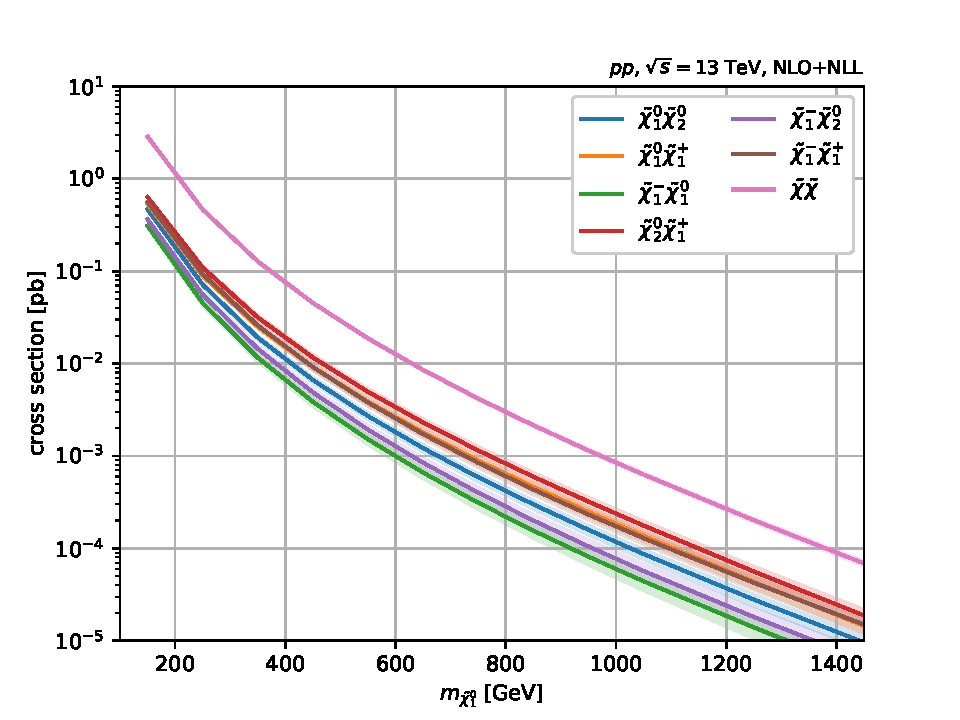
\includegraphics[width=0.7\textwidth]{images/SUSY_EWK_xsecs_m.pdf}
  \caption{Sección eficaz de la producción de gauginos en función de la masa de \ninoone.}
  \label{fig:SUSY_xs}
\end{figure}

Las desintegraciones \ninotwo (\chinoonepm) se establecen 100 \% en \ninoone a través de un $ Z $ ($ W ^ {\pm} $) fuera de la cáscara, y el último tiene la fracción de ramificación SM. Las fracciones de ramificación de \ninoone se establecieron 33 \% en $ \gravino + \gamma$, 33 \% en $ \ gravino + Z $ y 33 \% en $ \ gravino + h^{0} $. Esto se hizo para tener una buena cantidad de estadísticas para todos los posibles estados finales, con el fin de volver a ponderar cada evento al estado final deseado. Favorecer (o desfavorecer) un modelo con una \ninoone caracterizada con una fracción de ramificación particular a $\gamma$, $ Z $ o $ h^{0} $ ($ \text{BR}_{\gamma}, \text{BR}_{Z}, \text{BR}_{h^{0}} $), los eventos se ponderaron según:


\begin{equation}
	w  = [w_{\gamma\gamma}, w_{\gamma Z}, w_{\gamma h^{0}}, w_{ZZ}, w_{Zh^{0}}, w_{h^{0}h^{0}}] = 9 \cdot [\text{BR}_{\gamma}^{2}, \text{BR}_{\gamma}\cdot\text{BR}_{Z}, \text{BR}_{\gamma}\cdot\text{BR}_{h^{0}}, \text{BR}_{Z}^{2}, \text{BR}_{Z}\cdot\text{BR}_{h^{0}}, \text{BR}_{h^{0}}^{2}]
\end{equation}

Se estudiaron dos modelos particulares siguiendo ejemplos previos de análisis. El modelo fue la \ninoone decae 50 \% a $ \gamma + \gravino $ y 50 \% a $ Z + \gravino $ ($ w = \frac{9}{4} [1, 1, 0, 1, 0, 0] $) llamado 'modelo ph + Z', y el modelo donde \ninoone decae 50 \% a $ \gamma + \gravino $ y 50 \% a $ h^{0} + \gravino $ ($ w = \frac{9}{4} [1, 0, 1, 0, 0, 1] $) el llamado 'modelo ph + h'. Las \Cref{fig:met_srd200,fig:metmeff_metsig_srd200} muestran las distribuciones de \met, \met/\meff y \met\ significance para distintos puntos de señal, en comparación con las distribuciones de fondo, en una región sensible a bajas masas de \ninoone.

\begin{figure}
\centering
  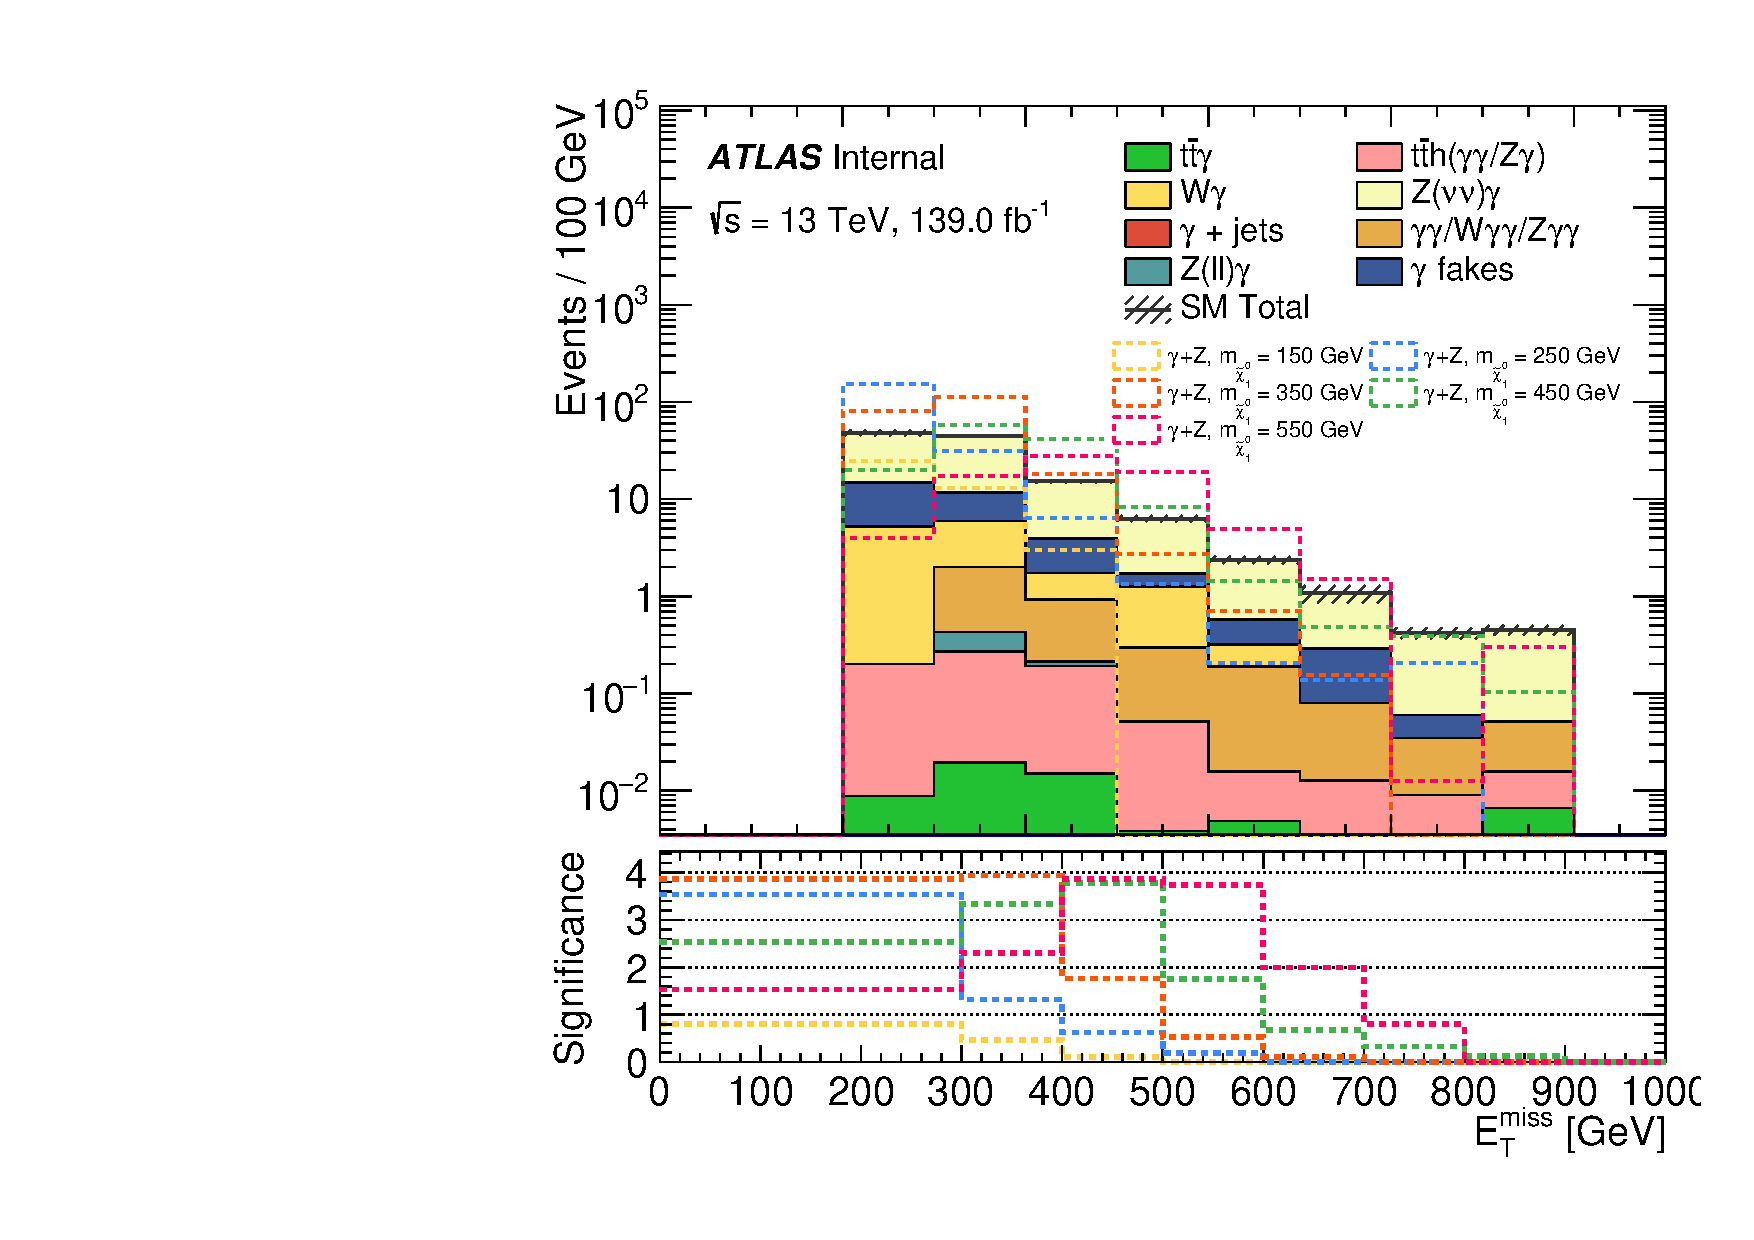
\includegraphics[width=0.6\textwidth]{images_tmp/can_SRd_200_met_et_afterFit.pdf}
  \caption{Distribución de \met\ para la región de señal de baja masa.}
  \label{fig:met_srd200}
\end{figure}


\begin{figure}
\centering
  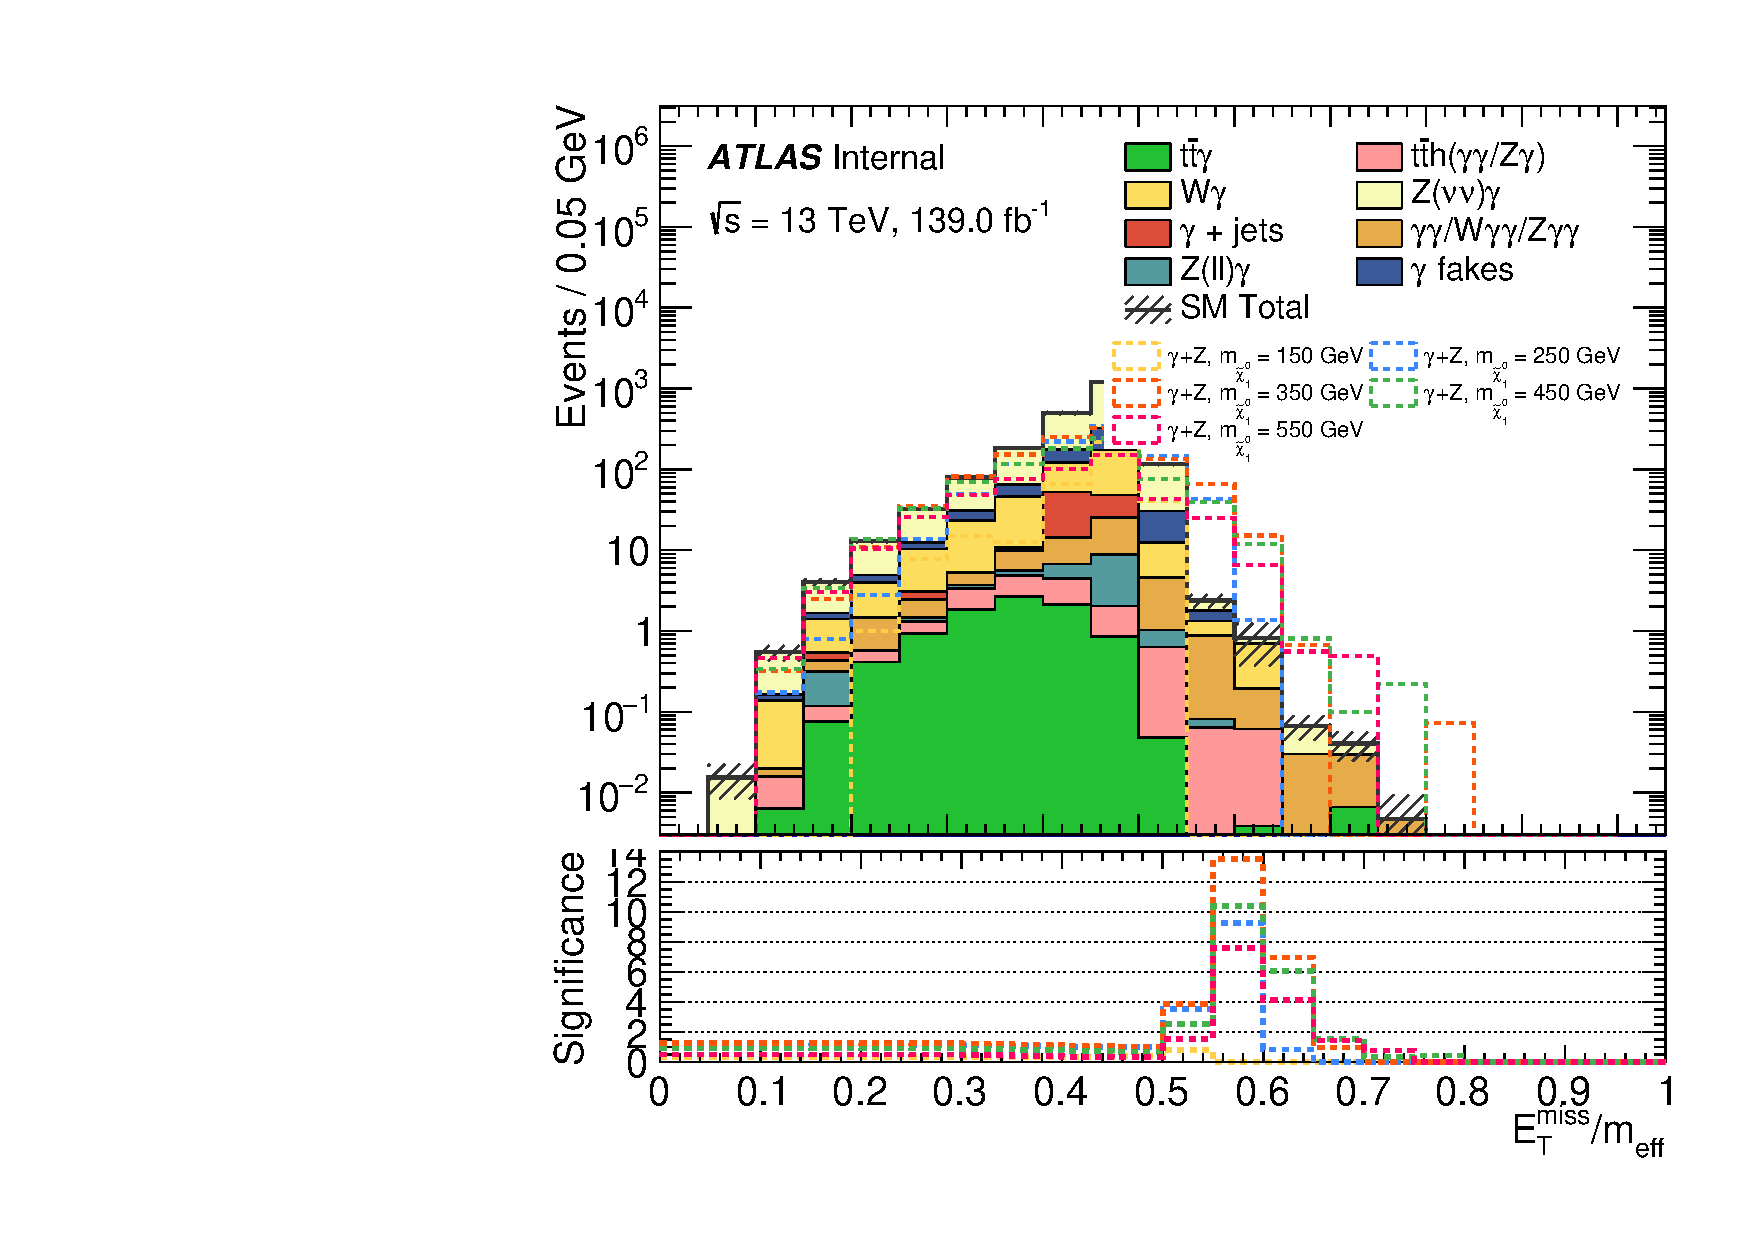
\includegraphics[width=0.4\textwidth]{images_tmp/can_SRd_200_met_etmeff_afterFit.pdf}%
  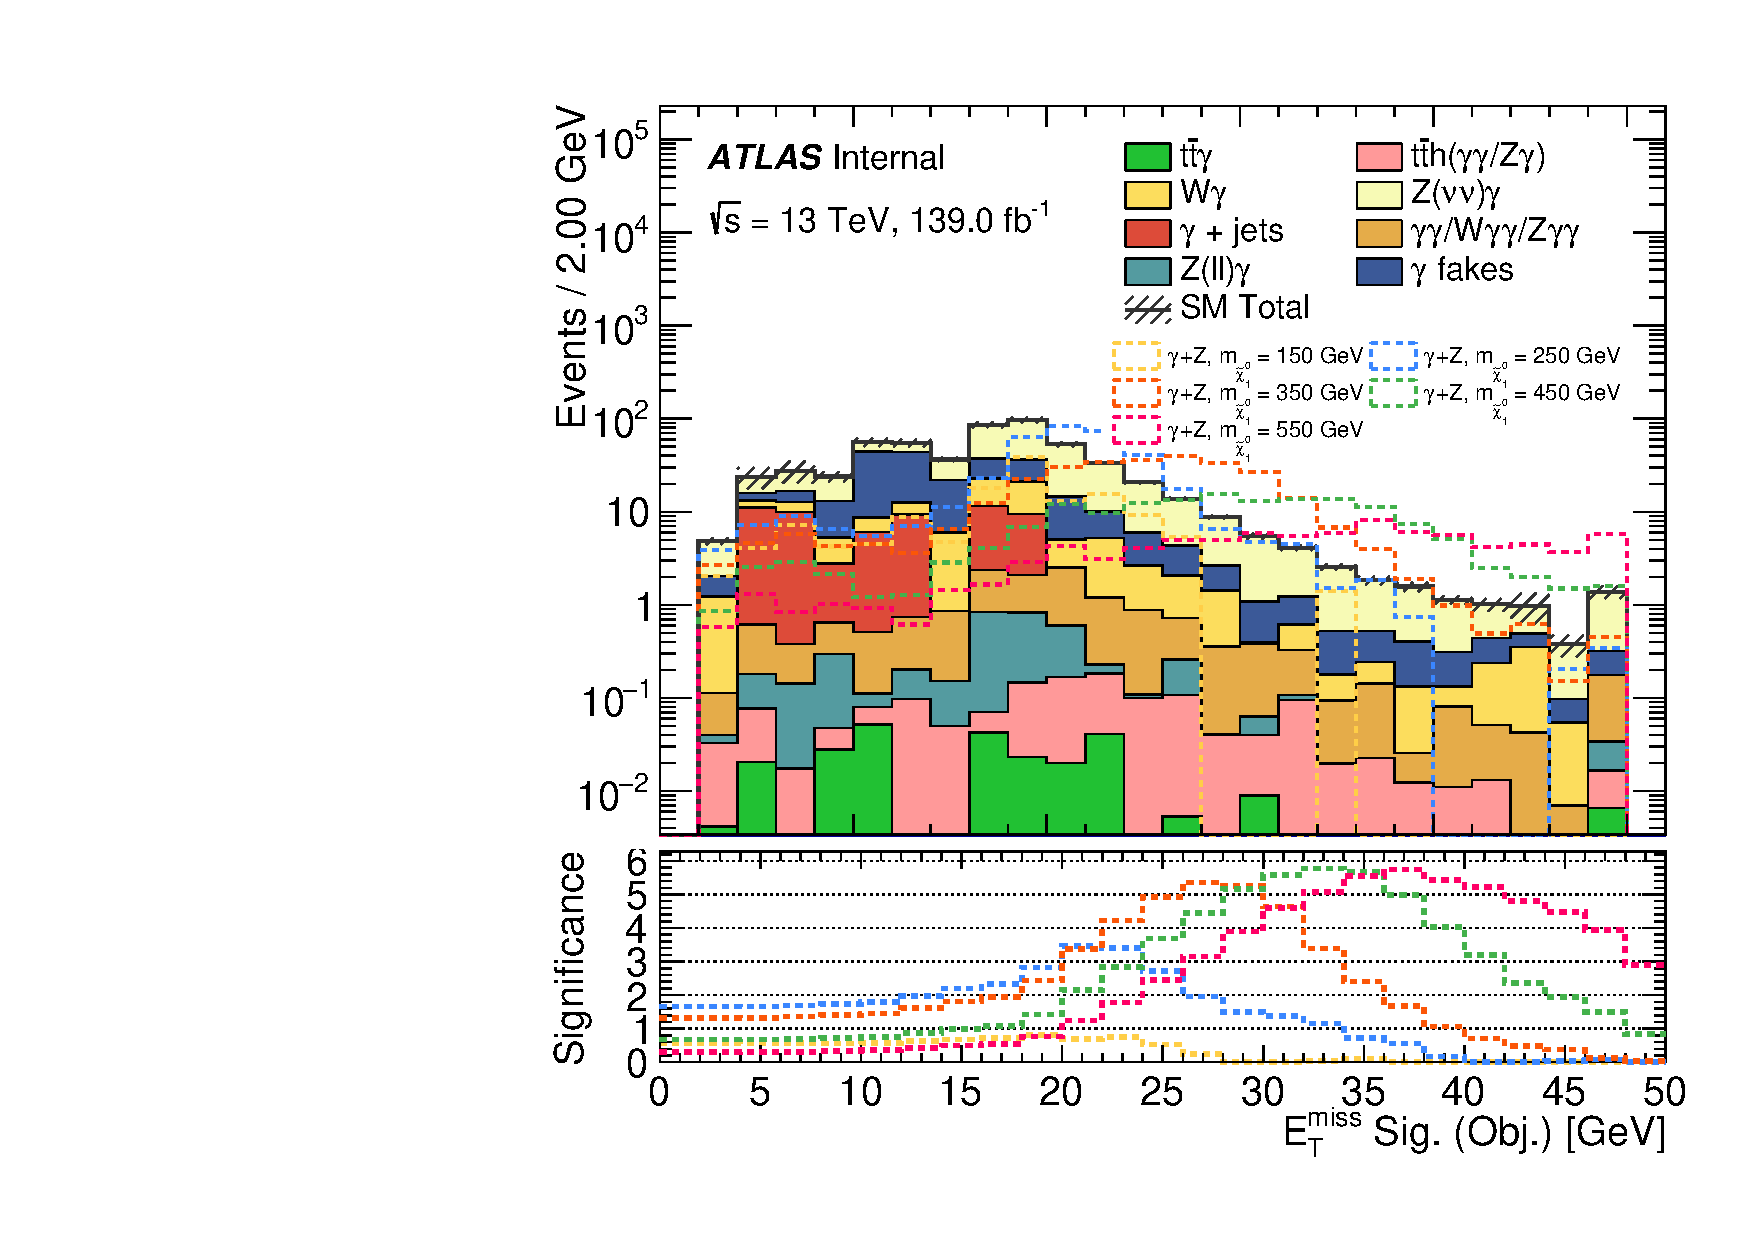
\includegraphics[width=0.4\textwidth]{images_tmp/can_SRd_200_met_sig_obj_afterFit.pdf}
  \caption{Distribución de \met/\meff (izquierda) y \met\ significance para la región de señal de baja masa.}
  \label{fig:metmeff_metsig_srd200}
\end{figure}